\documentclass[10pt,xcolor=pdflatex,hyperref={unicode}]{beamer}
\usepackage{newcent}
\usepackage[utf8]{inputenc}
\usepackage[czech]{babel}
\usepackage[T1]{fontenc}
\usepackage{hyperref}
\usepackage{fancyvrb}
\usetheme{FIT}
\usepackage{listings}

\lstdefinelanguage{Gherkin}{
	morekeywords = {
		Given,
		When,
		Then,
		And,
		Scenario,
		Feature,
		But,
		Background,
		Scenario Outline,
		Examples
	},
	sensitive=true,
	morecomment=[l]{\#},
	morestring=[b]",
	morestring=[b]'
}

%%%%%%%%%%%%%%%%%%%%%%%%%%%%%%%%%%%%%%%%%%%%%%%%%%%%%%%%%%%%%%%%%%
\title[Martin Krajňák - SEP]{Automatické generování testů pro GNOME GUI aplikace z metadat AT-SPI}

\author[]{Bc. Martin Krajňák}

\institute[]{

}
\institute[]{
xkrajn02@fit.vutbr.cz
\\
Vedúci práce: prof. Ing. Tomáš Vojnar, Ph.D. 
\\
Zadávateľ:   Red Hat Czech s.r.o.}

%\institute[]{Fakulta informačních technologií
%Vysokého učení technického v Brně\\
%Bo\v{z}et\v{e}chova 1/2. 612 66 Brno - Kr\'alovo Pole\\
%login@fit.vutbr.cz}

% České logo - Czech logo
% beamerouterthemeFIT.sty řádek 9: fitlogo1_cz

% \date{January 26, 2020}
\date{\today}
%\date{} % bez data / without date

%%%%%%%%%%%%%%%%%%%%%%%%%%%%%%%%%%%%%%%%%%%%%%%%%%%%%%%%%%%%%%%%%%

\begin{document}

\frame[plain]{\titlepage}

\begin{frame}\frametitle{Cieľ práce}
   
    
    \begin{block}{\vspace{2mm}\textbf{Nástroj na automatické generovanie automatizovaných testov}\vspace{2mm}}

    \begin{itemize}
    \item \textbf{Systematické vytvorenie testov na základe dostupných vykonateľných akcií GUI aplikácie}
    \vspace{5mm}
    \item \textbf{Využitie vstavenej podpory asistenčných technológii pre GTK/GNOME aplikácie}
    \vspace{5mm}
    \item \textbf{Využitie technológie OCR}
    \begin{itemize}
        \item \emph{rozpoznávanie znakov/textu z obrázkov}
    \end{itemize}
    \vspace{5mm}
    \item \textbf{Zjednodušenie/zrýchlenie procesu vývoja a údržby automatizovaných testov}
    \vspace{5mm}
    \item \textbf{Rýchle zistenie závažných chýb} 
    \end{itemize}

    \end{block}
\end{frame}

\begin{frame}\frametitle{Technológia AT-SPI a jej rozhrania}
    \begin{itemize}
        \item \textbf{AT-SPI je hlboko vstavaná do frameworku GTK, prítomná vo všetkých aplikáciach využívajúce grafické prvky GTK, prípadne ich varianty}
        \vspace{5mm}

        \item \textbf{AT-SPI ponúka strom prvkov aplikácie a ich:}
        \emph{\begin{itemize}
            \item \emph{pozíciu}
            \item \emph{viditeľnosť}
            \item \emph{vykonateľné udalosti/akcie}
            \item \emph{viditeľný text}
        \end{itemize}}
        \vspace{5mm}
        \item \textbf{Dostupnosť AT-SPI prvkov v jazyku Python3 cez knižnice:}
        \begin{itemize}
            \item \emph{pyatspi}
            \item \emph{dogtail}
        \end{itemize}
    \end{itemize}
\end{frame}

\begin{frame}\frametitle{Technológia AT-SPI - aplikácia Nautilus}
    \begin{figure}[h]
        \center{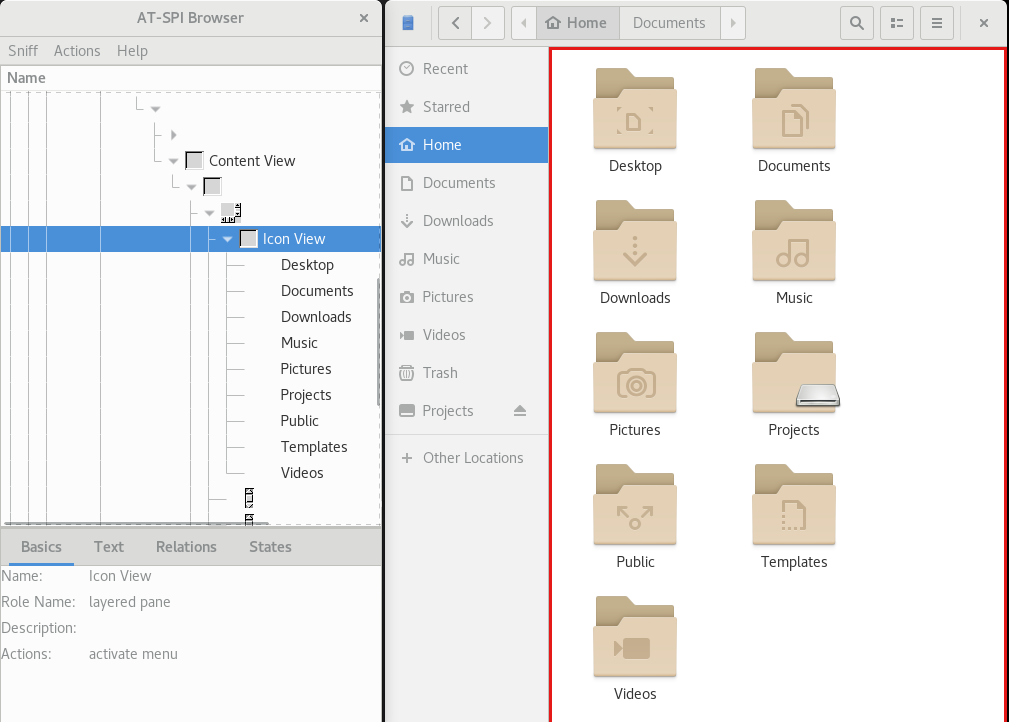
\includegraphics[scale=0.3]{img/sniff.png}}
        \label{sniff}
    \end{figure}
\end{frame}


\begin{frame}\frametitle{Extrakcia modelu, Generovanie testov}
\begin{enumerate}
    \item \textbf{Vytvorenie abstraktného modelu na základe dát AT-SPI:}
        \begin{enumerate}
        \item \emph{spustenie aplikácie}
        \item \emph{zmapovanie udalostí dostupných v súčasnom stave}
        \item \emph{postupné vytvorenie grafu udalostí (Event Flow graph)}
    \end{enumerate}
    \vspace{5mm}
    \item \textbf{Výber a vykonanie udalosti cez rozhrania AT-SPI}
    \vspace{5mm}
    \item \textbf{Overovanie stavu aplikácie}
    \begin{itemize}
        \item \emph{sledovanie chýb, kontrola behu, detekcia nových okien}
        \item \emph{kontrola zobrazenia určitých prvkov cez AT-SPI, OCR}
    \end{itemize}
    \vspace{5mm}
    \item \textbf{Vygenerovanie kroku testu \textit{(behave step)}}
\end{enumerate}

    \begin{figure}[h]
        \center{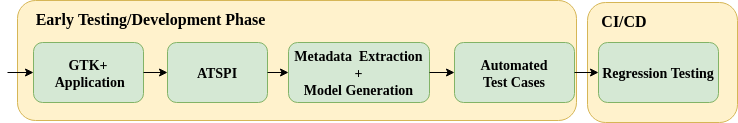
\includegraphics[scale=0.42]{img/diagram.png}}
        \label{diagram}
    \end{figure}
\end{frame}


\begin{frame}\frametitle{Výzvy}
    \textbf{\begin{itemize}
        \item určenie optimálneho konca testu (dĺžky sekvencie udalostí)
        \vspace{5mm}
        \item vyhodnotenie pokrytia udalostí testami
        \vspace{5mm}
        \item detekcia a začlenenie novo vzniknutých časti stromu počas generovania
        \vspace{5mm}
        \item reakcie na chyby počas generovania/označenie chyby aby sa jej generátor vyhol
    \end{itemize}
    }
\end{frame}

\begin{frame}[fragile]\frametitle{Ukážka jednoduchého testu - baobab}

\begin{lstlisting}[language=Gherkin]

Feature: Start and stop baobab in different ways

  @startViaCommand
  Scenario: Start via command
    Given Start baobab via command in session
    Then baobab should start
\end{lstlisting}
\begin{figure}[h]
    \center{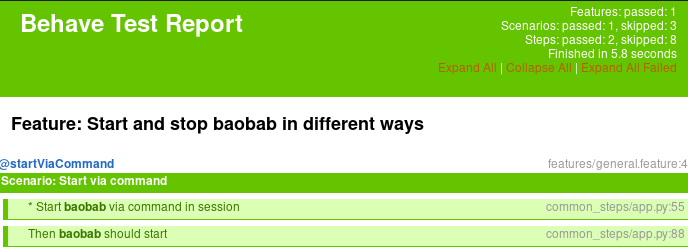
\includegraphics[scale=0.42]{img/behave_report.png}}
    \label{diagram}
\end{figure}

\end{frame}


\bluepage{
Ďakujem za pozornosť
}

\end{document}
